%
% The first command in your LaTeX source must be the \documentclass command.
% \documentclass[acmtog]{acmart}
\documentclass[sigchi]{acmart}
\settopmatter{printacmref=false}
\settopmatter{printacmref=false}
\setcopyright{none}
\settopmatter{printacmref=false} % Removes citation information below abstract
\renewcommand\footnotetextcopyrightpermission[1]{} % removes footnote with conference information in first column
\pagestyle{plain} % removes running headers
\renewcommand\footnotetextcopyrightpermission[1]{}

%%\usepackage{color}
\usepackage[usenames,dvipsnames,svgnames,table]{xcolor}
%
% defining the \BibTeX command - from Oren Patashnik's original BibTeX documentation.
% \def\BibTeX{{\rm B\kern-.05em{\sc i\kern-.025em b}\kern-.08emT\kern-.1667em\lower.7ex\hbox{E}\kern-.125emX}}
%
% The majority of ACM publications use numbered citations and references. If you are preparing content for an event
% sponsored by ACM SIGGRAPH, you must use the "author year" style of citations and references. Uncommenting
% the next command will enable that style.
%\citestyle{acmauthoryear}
%
% end of the preamble, start of the body of the document source.

\begin{document}

%
% The "title" command has an optional parameter, allowing the author to define a "short title" to be used in page headers.
\title{    
	Project 5: Collaboration and Competition\\
	{\large Udacity Deep Reinforcement Learning Nanodegree Program}
}

%
% The "author" command and its associated commands are used to define the authors and their affiliations.
% Of note is the shared affiliation of the first two authors, and the "authornote" and "authornotemark" commands
% used to denote shared contribution to the research.
\author{Bob Flagg}\affiliation{}

%
% By default, the full list of authors will be used in the page headers. Often, this list is too long, and will overlap
% other information printed in the page headers. This command allows the author to define a more concise list
% of authors' names for this purpose.
\renewcommand{\shortauthors}{Bob Flagg}

%
% The abstract is a short summary of the work to be presented in the article.

%
% The code below is generated by the tool at http://dl.acm.org/ccs.cfm.
% Please copy and paste the code instead of the example below.
%

%
% A "teaser" image appears between the author and affiliation information and the body 
% of the document, and typically spans the page. 
\begin{teaserfigure}
	\centering
  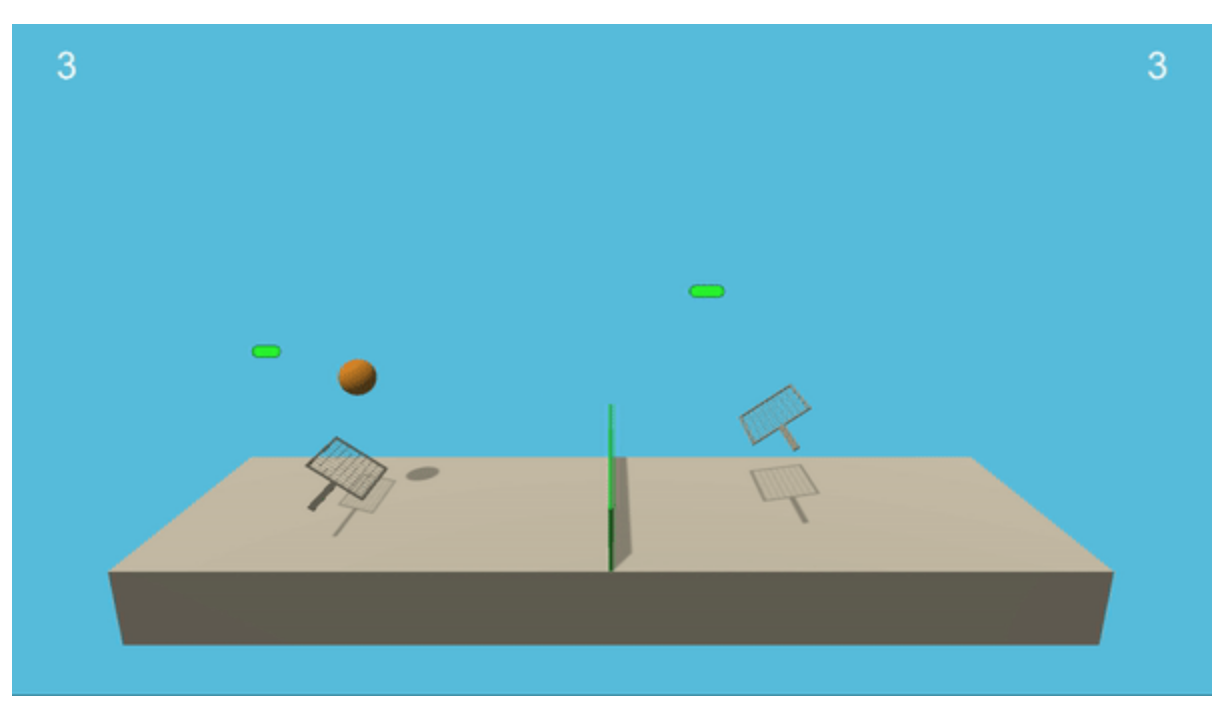
\includegraphics[width=0.4\textwidth]{teaser}
  \caption{}
  \label{fig:teaser}
\end{teaserfigure}

%
% This command processes the author and affiliation and title information and builds
% the first part of the formatted document.
\maketitle

%%%%%%%%%%%%%%%%%%%%%%%%%%%%%%%%%%%%%%%%%%%%%%%%%%%%%%%%%%%%%%
%% Introduction                                                                                                                             %%
%%%%%%%%%%%%%%%%%%%%%%%%%%%%%%%%%%%%%%%%%%%%%%%%%%%%%%%%%%%%%%
\section{Introduction}

In this project I'll implement two solutions to the 
\href{https://github.com/Unity-Technologies/ml-agents/blob/master/docs/Learning-Environment-Examples.md#tennis}{\underline{Tennis}}
environment from the 
\href{https://unity3d.ai}{\underline{Unity Machine Learning Toolkit}}.
This is a multi-agent environment, where two agents control rackets to bounce a ball over a net. If an agent hits the ball over the net, it receives a reward of +0.1.  If an agent lets a ball hit the ground or hits the ball out of bounds, it receives a reward of -0.01.  Thus, the goal of each agent is to keep the ball in play.

The observation space consists of 8 variables corresponding to the position and velocity of the ball and racket. Each agent receives its own, local observation.  Two continuous actions are available, corresponding to movement toward (or away from) the net, and jumping. 

The task is episodic, and in order to solve the environment, your agents must get an average score of +0.5 (over 100 consecutive episodes, after taking the maximum over both agents). Specifically,
\begin{itemize}
	\item  After each episode, we add up the rewards that each agent received (without discounting), to get a score for each agent. This yields 2 (potentially different) scores. We then take the maximum of these 2 scores.
	\item  This yields a single \textbf{score} for each episode.
\end{itemize}
The environment is considered solved, when the average (over 100 episodes) of those \textbf{scores} is at least +0.5.



I'll use 
{\em Deep Deterministic Policy Gradient}~\cite{Silver:2014:DPG:3044805.3044850} (DDPG) 
and
{\em Multi-Agent Deep Deterministic Policy Gradient}~\cite{DBLP:journals/corr/LoweWTHAM17} (MADDPG) 
to solve the environment.
Source code in Python, using PyTorch, is available 
in the  
\href{https://github.com/bobflagg/Collaboration-and-Competition}{\underline{Collaboration and Competition}}
repo.





\section{Background}

The 
\href{https://github.com/Unity-Technologies/ml-agents/blob/master/docs/Learning-Environment-Examples.md#tennis}{\underline{Tennis}}
environment is a {\em sequential decision making problem}, in which two agents interact with each other and their environment over discrete time
steps and try to find {\em policies} to maximize the expected {\em discounted return}:
$$G_t = \sum_{k=0}^{\infty}\gamma^kR_{t+k+1},$$
where $\gamma\in[0,1]$  is a discount factor that trades-off the importance of immediate and future rewards.
See~\cite{DBLP:books/lib/SuttonB98} for a general discussion of this sort of problem. 

In this project I will use policy-based methods, which try to directly  find an {\em optimal policy}, $\pi^*$, each agent can use to decide what actions to take. 

\subsection{Deep Deterministic Policy Gradient}

In my first solution, I'll use 
 {\em Deep Deterministic Policy Gradient}~\cite{Silver:2014:DPG:3044805.3044850} (DDPG),
which is motivated by an important connection between the action selected by an optimal policy and the {\em optimal action-value function} 
	$$Q^*(s, a) =  \max_{\pi}Q^{\pi}(s,a).$$
Namely, if you know the optimal action-value function, then in any given state, $s$, an optimal action can be found by solving
	 $$\pi^*(s) = \arg\max_a Q^*(s,a).$$
 DDPG concurrently learns an approximator to $Q^*(s,a)$ and an approximator to $\pi^*(s)$, and it does so in a way which is specifically adapted for environments with continuous action spaces. 

\subsubsection{Learning $Q^*(s,a)$}

The starting point for approximating the action value function is the \textbf{Bellman Equation}:
$$Q^{*}(s,a) = \mathbb{E}\big[R_{t+1}+\gamma\cdot \max_{a'}Q^{*}(S_{t+1},a')| S_t = s, A_t=a\big].$$
Suppose we are approximating $Q^*(s, a)$ with a neural network, $Q_\phi(s,a)$, and we have collected a set $\mathcal{D}$ of
transitions $(s, a, r, s', d)$, then the \textbf{mean-squared Bellman error} (MSBE)
		$$L(\phi, \mathcal{D}) = \mathbb{E}_{\mathcal{D}}\big[\big(Q_\phi(s,a)-(r+\gamma\cdot(1-d)\max_{a'}Q_\phi(s',a'))\big)^2\big]$$
tells us roughly how closely $Q_{\phi}$ comes to satisfying the Bellman equation and so can serve as the loss function in tuning $\phi$.

\subsubsection{Learning $\pi^*(s)$}

Learning the optimal policy is pretty simple: we want to learn a deterministic policy $\pi^*(s)$ which gives the action that maximizes $Q^*(s, a)$.
For this DDPG uses a neural network, $\pi_\theta(s)$, and loss function
$$L(\theta, \mathcal{D}) = -\mathbb{E}_{\mathcal{D}}\big[Q_\phi(s,\pi_\theta(s))\big].$$
 
\subsection{Multi-Agent Actor-Critic}

In my second solution, I'll use {\em Multi-Agent Deep Deterministic Policy Gradient}~\cite{DBLP:journals/corr/LoweWTHAM17} (MADDPG).  

\begin{figure}[h]
	\centering
	\includegraphics[width=3.0in]{multi-agent-actor-critic}
	\label{fig:ma-ac}
	\caption{Multi-Agent Actor-Critic~\cite{DBLP:journals/corr/LoweWTHAM17}}
\end{figure}

As illustrated in Figure 2, the key idea of MADDPG is to use \textbf{centralized critics}, which observe all states and actions, and 
 \textbf{decentralized actors}, which only observe their own state.
 

\section{Playing Tennis with DDPG}

In the DDPG solution to the 
\href{https://github.com/Unity-Technologies/ml-agents/blob/master/docs/Learning-Environment-Examples.md#tennis}{\underline{Tennis}}
environment I train a single agent that plays against itself. The code is in the 
\href{https://nbviewer.jupyter.org/github/bobflagg/Collaboration-and-Competition/blob/master/01-Playing-Tennis-with-DDPG.ipynb}{\underline{Playing Tennis with DDPG notebook}}.

The key components and hyper-parameter settings are outlined below.
\begin{itemize}
	\item \textbf{Actor Network}: One fully connected linear hidden layer with 256 units. The input size is equal to the environment state-size and the output size is equal to the environment action-size. It uses ReLu activation functions and batch normalization after the hidden layer.
	\item \textbf{Critic Network}: Three fully connected linear hidden layers. The first hidden layer has 256 units and has input size equal to the environment state-size. The second hidden layer has 256 units and input size equal to 256 + the environment action-size. The third hidden layer has 128 units. ReLu activation functions are used throughout  and batch normalization is applied after the first layer. The output of this network is one-dimensional.
	\item \textbf{Hyperparameter Settings}: 
	I trained for 1,500 episodes with a batch size of 128, discount factor of $\gamma = 0.99$, soft update weight of $\tau = 0.001$, actor learning rate of $0.0001$, 
	 and critic learning rate of $0.001$.  To get DDPG to learn in a multi-agent environment I had to separate updating network parameters from adding samples to the replay buffer so that I could interleave these two steps in an appropriate proportion. After a bit of experimentation, I chose to update the networks 30 times after every 10 timesteps. 
\end{itemize}

With the above settings I achieved an average score of 0.68 for the final 100 episodes and even managed to get an average score above 0.8 briefly during training.

\begin{figure}[h]
	\centering
	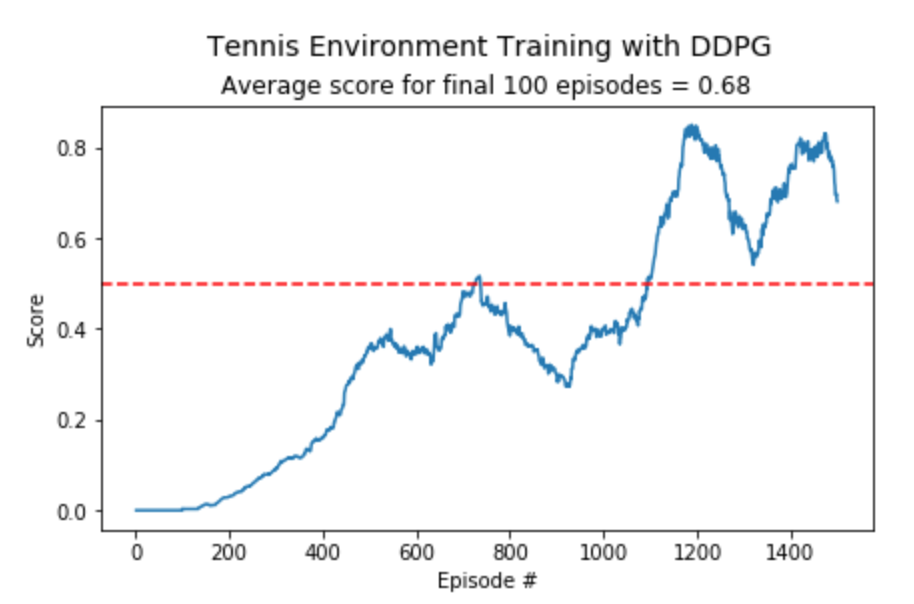
\includegraphics[width=3.0in]{ddpg-scores}
	\label{fig:ddpg-scores}
	\caption{DDPG Training Scores}
\end{figure}

\section{Playing Tennis with MADDPG}
The solution above is simple, stable and achieves a pretty high average score but it is not very satisfying from a multi-agent reinforcement learning point of view.  In general it will not be possible to use the same model instance for all agents since different agents may need to achieve different goals.
In the 
\href{https://nbviewer.jupyter.org/github/bobflagg/Collaboration-and-Competition/blob/master/02-Playing-Tennis-with-MADDPG.ipynb}{\underline{Playing Tennis with MADDPG notebook}}
 I address that shortcoming by adapting DDPG to the multi-agent setting as in the paper {\em Multi-Agent Deep Deterministic Policy Gradient}~\cite{DBLP:journals/corr/LoweWTHAM17} (MADDPG).   I was able to solve the tennis environment with this approach but the results were disappointing so I won't bother describing hyper-parameter settings here.  Figure 3 below shows the scores during training.  It's not really surprising that this approach does not do nearly as well as self-playing DDPG because it does not take advantage of special features of the Tennis environment but the average score did reach 0.52 so at least it solved the task.
\begin{figure}[h]
	\centering
	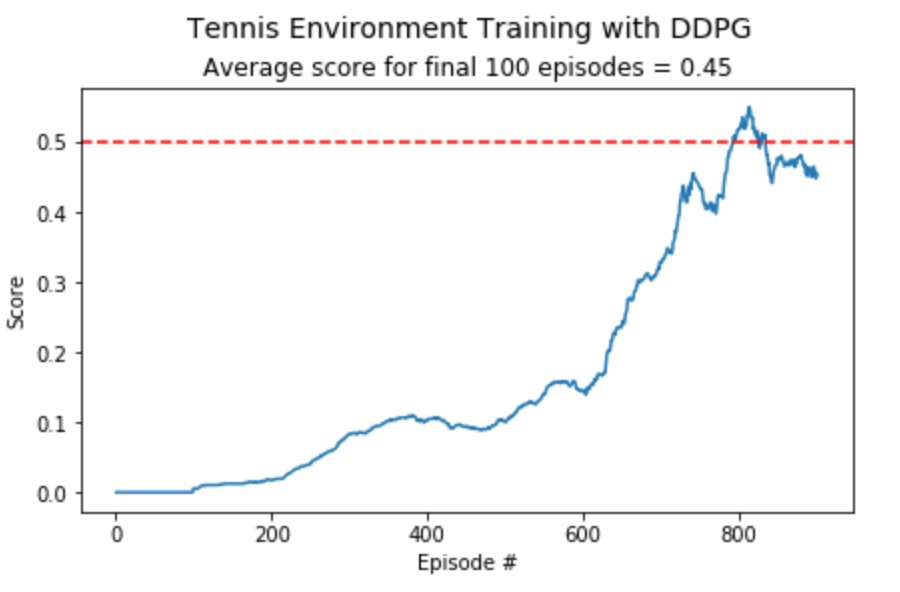
\includegraphics[width=3.0in]{ma-scores}
	\label{fig:ddpg-scores}
	\caption{MADDPG Training Scores}
\end{figure}

\section{Improving Performance}

Deep Deterministic Policy Gradient did well on this task.  To improve performance futher, I would do grid search on the hyper-parameters and network architectures for this approach.  Another interesting direction would modify the MADDPG agorithm by allowing each critic instance to know which agent it is criticizing; that is, feed the corresponding agent's observation and action into the netword separately from those of the other agents so the critic could focus on the appropriate agent's actions and observtions whild still having access to all observations and actions.

\bibliographystyle{ACM-Reference-Format}
%%\nocite{*}
\bibliography{report}


\end{document}

The specific policy-based method I'll used is called {\em Deep Deterministic Policy Gradient}~\cite{Silver:2014:DPG:3044805.3044850} (DDPG) which 
concurrently learns a policy and a Q-function. Recall that the {\em Q-function} for a policy $\pi$ is defined by
$$Q^{\pi}(s,a) = \mathbb{E}_\pi\big[G_t| S_t = s, A_t=a\big].$$
DDPG uses  off-policy data and the \textbf{Bellman Equation}:
$$Q^{\pi}(s,a) = \mathbb{E}_\pi\big[R_{t+1}+\gamma\cdot Q^{\pi}(S_{t+1},A_{t+1})| S_t = s, A_t=a\big].$$
to learn the Q-function, and uses the Q-function to learn the policy.

%%%%%%%%%%%%%%%%%%%%%%%%%%%%%%%%%%%%%%%%%%%%%%%%%%%%%%%%%%%%%%
%% Deep Q-Learning for Navigation                                                                                                %%
%%%%%%%%%%%%%%%%%%%%%%%%%%%%%%%%%%%%%%%%%%%%%%%%%%%%%%%%%%%%%%
\section{Soft Actor-Critic}

\subsection{Entropy-Regularized Reinforcement Learning}

$$\pi^* =  \operatorname{arg\,max}_{\pi}\mathbb{E}_{\tau\sim\pi}\big[\sum_{t=0}^{\infty}\gamma^t\big(R_t+\alpha \mathcal{H} [\pi(\cdot|S_t)]\big)\big].$$

$$L(\phi_i, {\mathcal D}) = \underset{(s,a,r,s',d) \sim {\mathcal D}}{\mathbb{E}}\left[
\Bigg( Q_{\phi_i}(s,a) - \left(r + \gamma (1 - d) V_{\psi_{\text{targ}}}(s') \right) \Bigg)^2
\right].$$

{\em Soft Actor-Critic Algorthm}~\cite{DBLP:journals/corr/abs-1812-05905}.
Source code in Python, using PyTorch, is available on 
\href{http://github.com}{\underline{github}} 
in the repo 
\href{https://github.com/bobflagg/Actor-Critic-for-Continuous-Control}{\underline{Actor-Critic-for-Continuous-Control}}.

For a policy $\pi$, the {\em state-value function}, $V^\pi$, is defined by
$$V^{\pi}(s) = \mathbb{E}_\pi\big[G_t| S_t = s\big].$$
and we would like to find $\pi$ so that 
$$V^{\pi}(s) = V^{*}(s) = \max_{\pi'}V^{\pi'}(s).$$



%%%%%%%%%%%%%%%%%%%%%%%%%%%%%%%%%%%%%%%%%%%%%%%%%%%%%%%%%%%%%%
%% Resources                                                                                                                               %%
%%%%%%%%%%%%%%%%%%%%%%%%%%%%%%%%%%%%%%%%%%%%%%%%%%%%%%%%%%%%%%
\section{Additional Resources}

\begin{enumerate}
	
	\item \href{https://blog.lateral.io/2017/10/text-segmentation-using-word-embeddings/}{\color{red}Text Segmentation using Word Embeddings}
	\item \href{http://www.cs.man.ac.uk/~mary/choif/software.html}{\color{red}Freddy Choi: Code and data for segmentation experiments}
	\item \href{https://github.com/datafordemocracy/topictiling}{\color{red}Repository that does topictiling on cable news}
	\item \href{https://github.com/logological/C99}{\color{red}C99, a domain-independent algorithm for linear text segmentation by Freddy Choi}
	\item \href{https://github.com/levy5674/text-tiling-demo}{\color{red}Demo of ntlk's TextTilingTokenizer}
	\item \href{http://politicaladarchive.org/data/}{\color{red}Political TV Ad Archive}
	\item \href{http://classif.ai/dataset/tv-news-channel-commercial-detection-dataset/}{\color{red}TV News Channel Commercial Detection Dataset}
	\item \href{http://github.com/alexalemi/segmentation}{\color{red}Alex Alemi: Code and data for segmentation experiments}
	
\end{enumerate}


